\section{testing}
\begin{itemize}
\item{The main goal of our testing approach is to test the more complex parts of game such as
trading. One of our goals is not to achieve 100 percent test coverage, but to test the complex parts
in a a nice way. }
    \item {
Our design is wel suited for testing. Since our design adheres to the dependency injection pattern
injecting mocked objects of classes is easy. For mocking we used the
Mockito\footnote{https://code.google.com/p/mockito/} framework.}
\item {Each of the three modules can be compiled and tested separately. However the \emph{bohnanza}
module is rather abstract and thus testing some abstract classes do not really make sense. We test
more concrete classes in either the \gls{std} module or the \gls{hb} module.}
\item {In the bohanza module we mainly tested whether the \texttt{Beanometer} or \texttt{CardList}
works correctly. This is shown in the coverage report in the package \texttt{bohnanza.game}. Since a
game can not really be played in the bohnanza module the gameplay is tested in a concrete
implementation of bohnanza, namely bohnanza-std. This is shown in the package
\texttt{bohnanza.gameplay}}.
\end{itemize}

\begin{figure}[h!]
    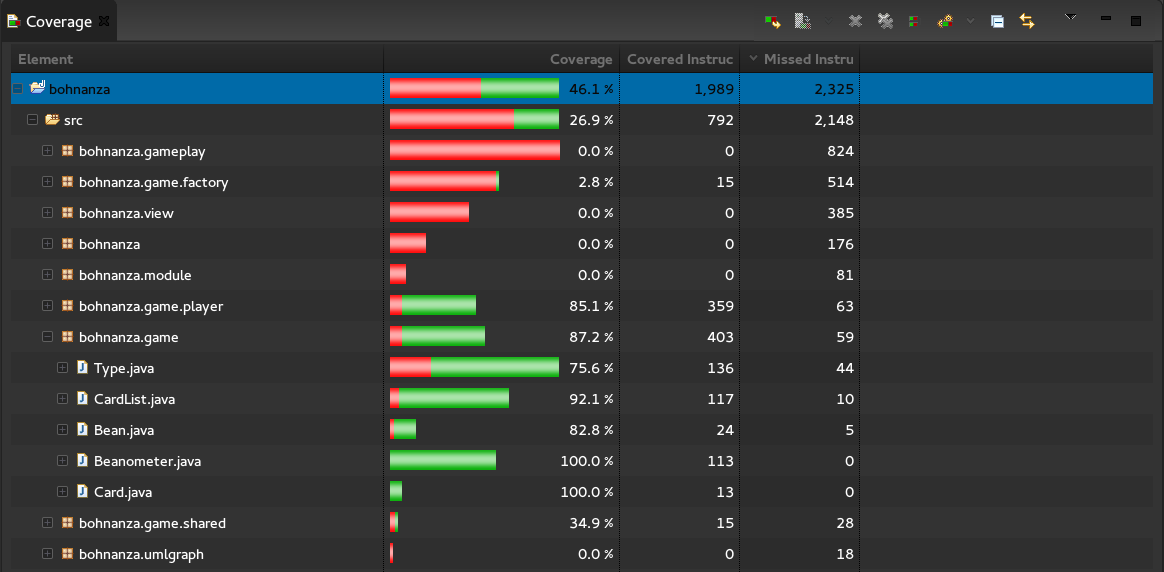
\includegraphics[width=\textwidth]{../img/coverage}
    \caption{Coverage of the \emph{bohnanza} module}
    \label{fig:test:coverage}
\end{figure}

\begin{figure}[h!]
    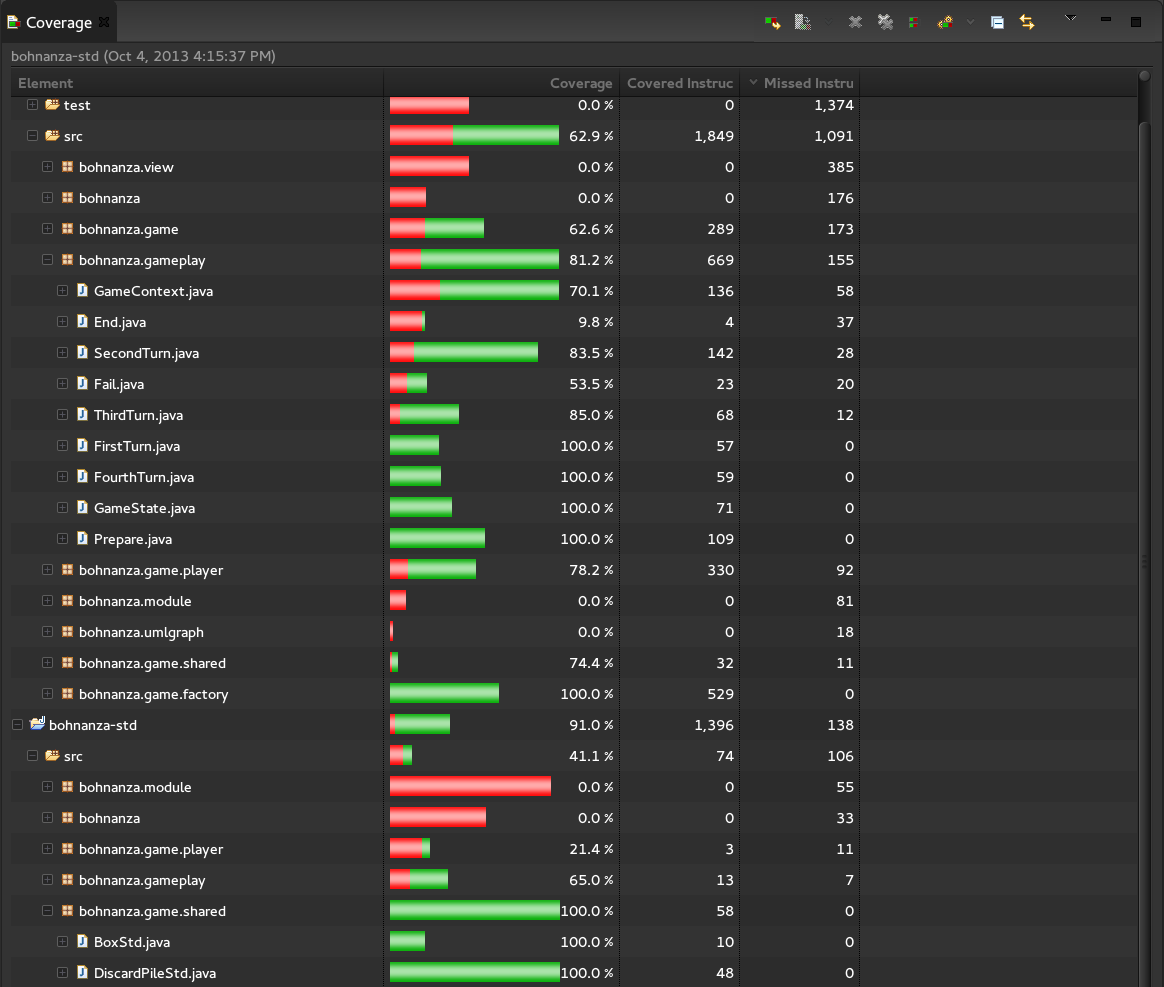
\includegraphics[width=\textwidth]{../img/coverage-std}
    \caption{Coverage of the \emph{bohanza-std} module}
    \label{fig:test:coverage-std}
\end{figure}
